% TOFTA — Player Mat (A4 landscape)
% Compile with:  pdflatex player_mat.tex   (or lualatex)
% Requires: texlive-latex-extra texlive-fonts-recommended

\documentclass{article}
\usepackage[
  paperwidth=297mm, paperheight=210mm,
  top=0mm, bottom=0mm, left=0mm, right=0mm
]{geometry}
\usepackage{tikz}
\usepackage{xcolor}
\usepackage[T1]{fontenc}
\usepackage{lmodern}
\usetikzlibrary{calc}
\pagestyle{empty}
\parindent=0pt

% ── Colour palette ────────────────────────────────────────────────────────────
\definecolor{clmilitary}{HTML}{c53030}
\definecolor{clmarket}{HTML}{276749}
\definecolor{clscience}{HTML}{553c9a}
\definecolor{clwonders}{HTML}{744210}
\definecolor{clmisc}{HTML}{4a5568}
\definecolor{panelbg}{HTML}{2d3748}
\definecolor{slotbg}{HTML}{edf2f7}
\definecolor{erabadge2}{HTML}{9b2c2c}
\definecolor{erabadge3}{HTML}{7b341e}
\definecolor{vpgold}{HTML}{d69e2e}
\definecolor{darkgrey}{HTML}{4a5568}
\definecolor{bodybg}{HTML}{f0f0f0}

% ── Building-track macro (called inside tikzpicture) ─────────────────────────
% Usage: \buildtrack{x-left mm}{TikZ colour name}{Track Name}{s1}{s2}{s3}{s4}
\newcommand{\buildtrack}[8]{%
  % coloured header
  \fill[#2!80] (#1,150) rectangle ($(#1,150)+(56,6)$);
  \draw[#2]    (#1,150) rectangle ($(#1,150)+(56,59)$);
  \node[font=\scriptsize\bfseries, text=white, anchor=west] at ($(#1,150)+(1,3)$) {#3};
  % 4 reward slots
  \foreach \si/\rl in {0/#4, 1/#5, 2/#6, 3/#7} {
    \pgfmathsetmacro{\slx}{#1 + 1 + \si * 13.5}
    \fill[#2!15] (\slx,157) rectangle ($(\slx,157)+(12,14)$);
    \draw[#2!60, thin] (\slx,157) rectangle ($(\slx,157)+(12,14)$);
    \node[font=\tiny, text=#2!70!black, anchor=center] at ($(\slx,157)+(6,7)$) {\rl};
    \fill[white] ($(\slx,157)+(6,19)$) circle (3mm);
    \draw[#2, thin] ($(\slx,157)+(6,19)$) circle (3mm);
  }
  % connector line between circles
  \draw[#2!40, thin] ($(#1,157)+(7,19)$) -- ($(#1,157)+(49,19)$);
}

% ── Section header bar macro ──────────────────────────────────────────────────
% \secbar{x}{y}{w}{colour}{label}
\newcommand{\secbar}[5]{%
  \fill[#4] (#1,#2) rectangle ($(#1,#2)+(#3,5)$);
  \node[font=\scriptsize\bfseries, text=white, anchor=west] at ($(#1,#2)+(1,2.5)$) {#5};
}

\begin{document}
% ── Canvas: x=1mm right, y=1mm DOWN from top-left ────────────────────────────
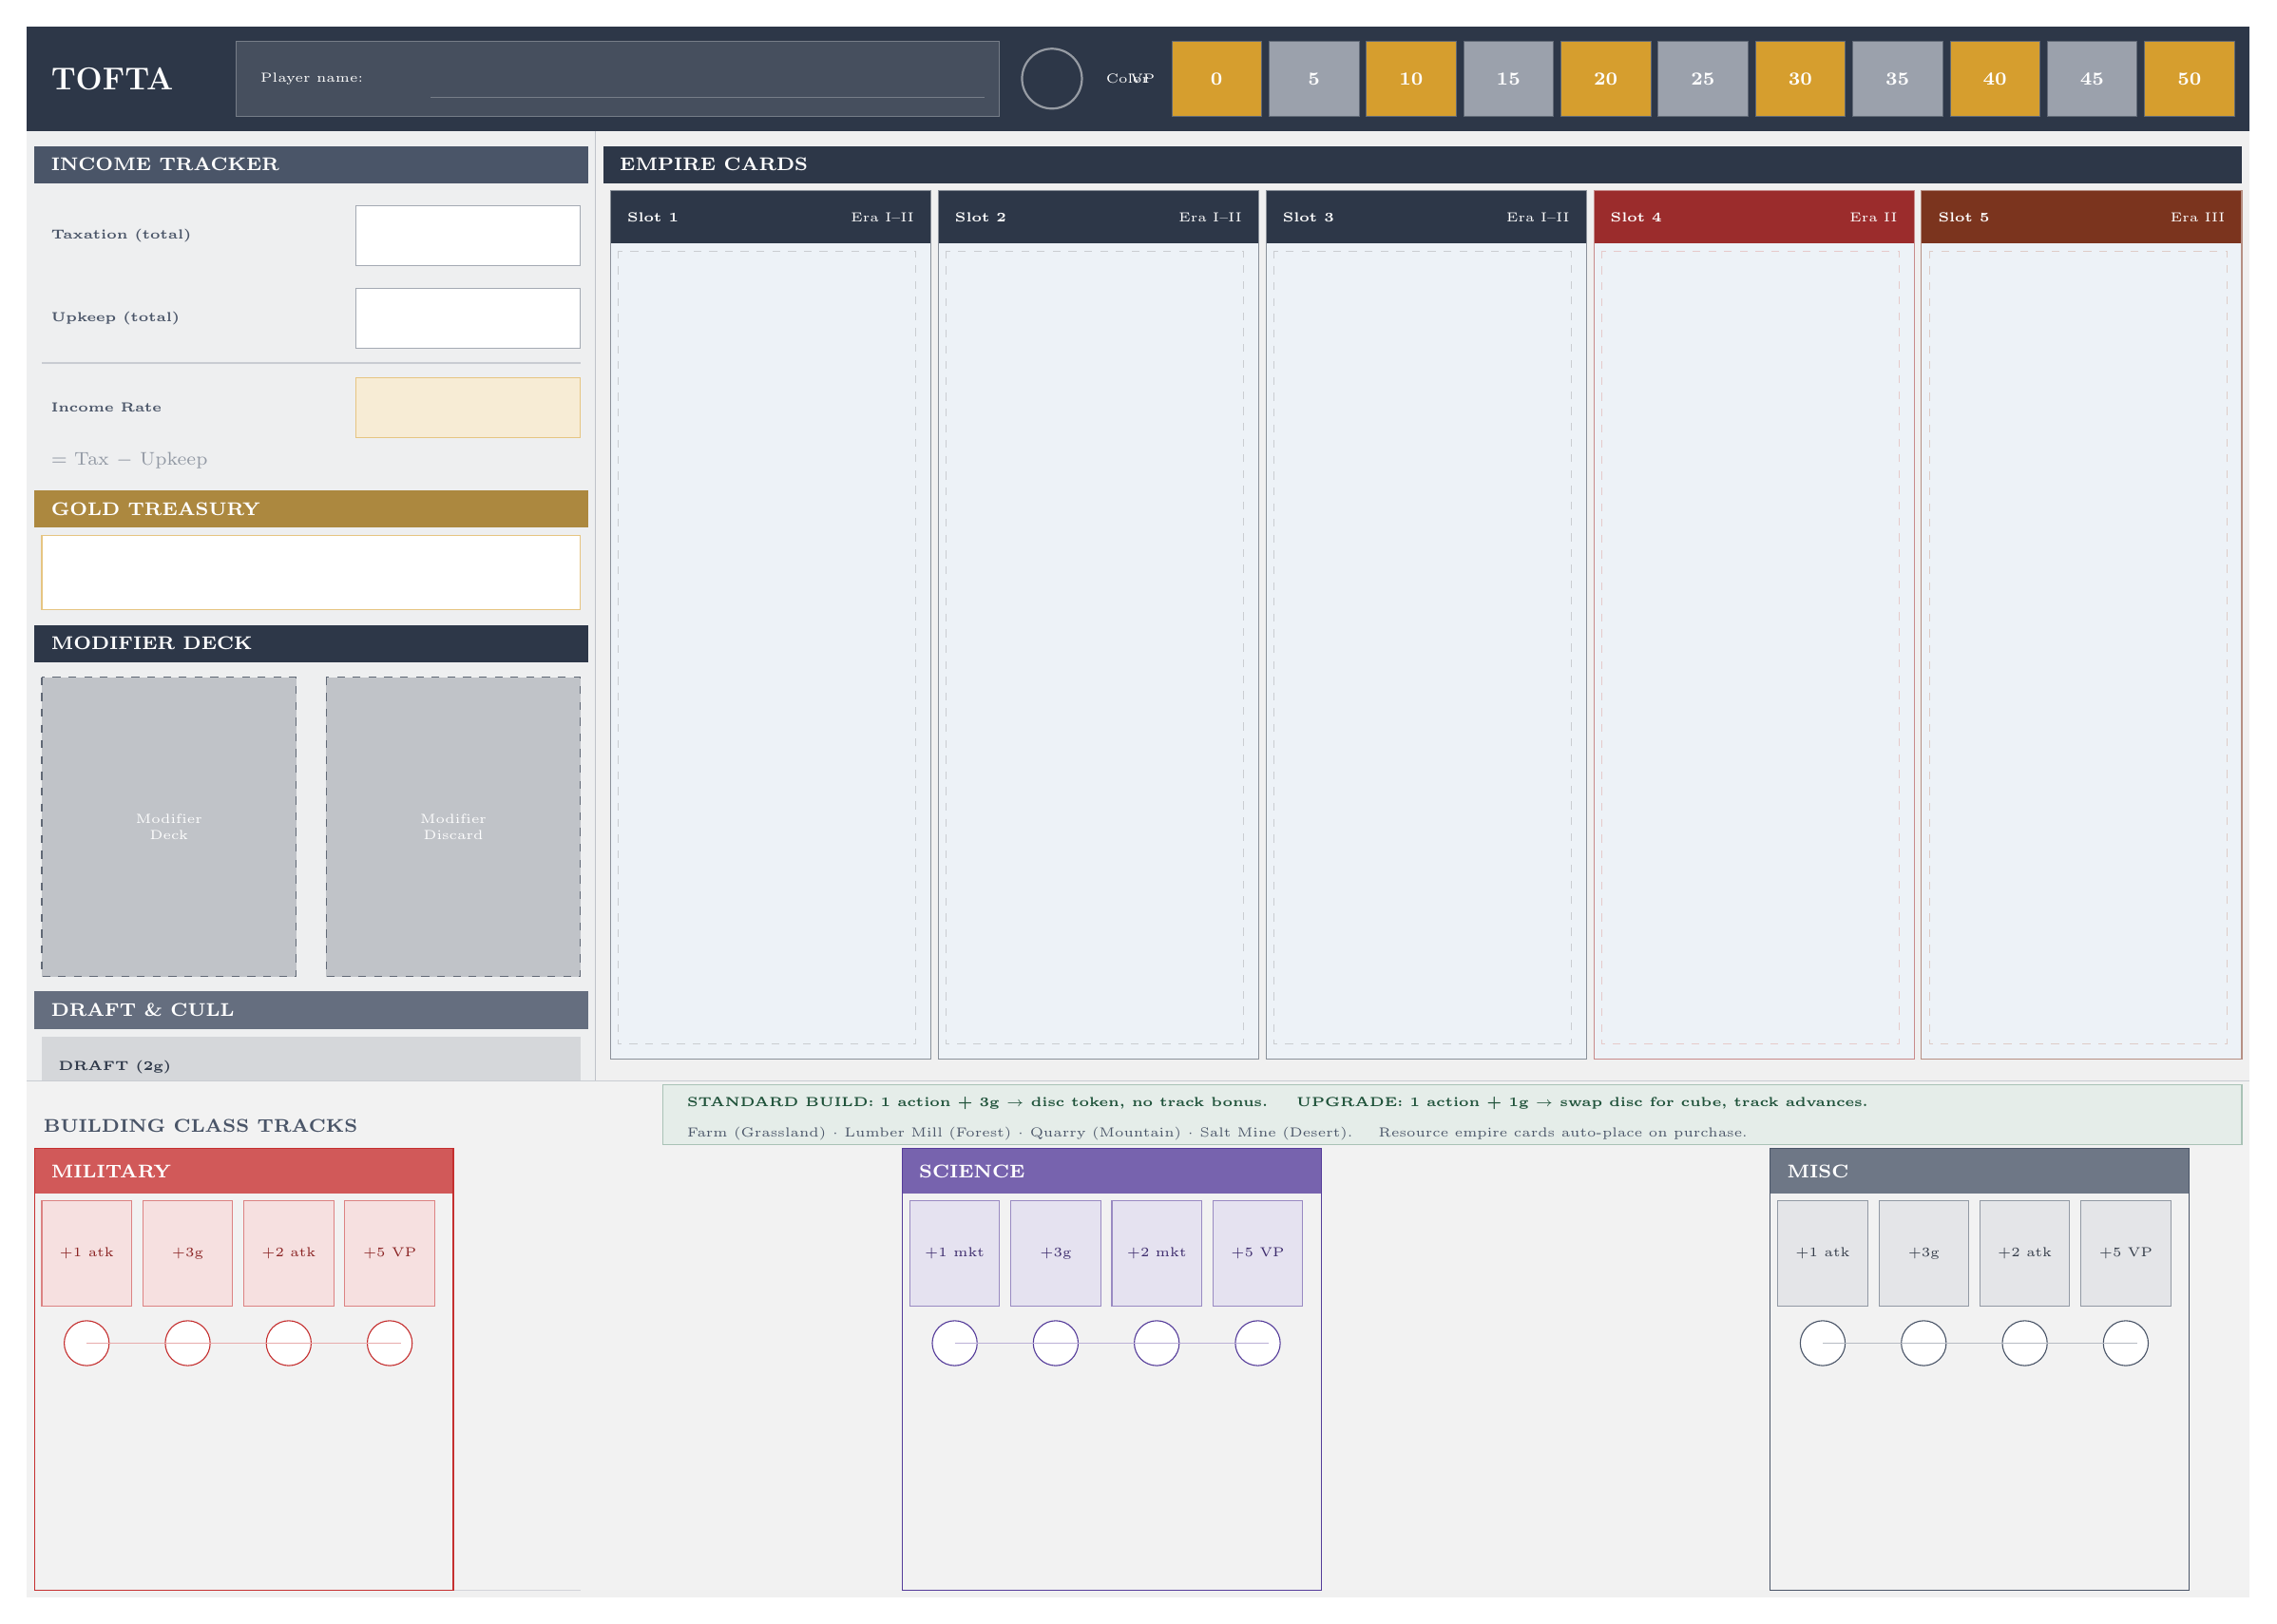
\begin{tikzpicture}[x=1mm, y=-1mm, shift={(0mm, 210mm)}]

  % ── Background ─────────────────────────────────────────────────────────────
  \fill[bodybg] (0,0) rectangle (297,210);

  % ════════════════════════════════════════════════════════════════════════════
  % HEADER  y 0–14
  % ════════════════════════════════════════════════════════════════════════════
  \fill[panelbg] (0,0) rectangle (297,14);

  \node[font=\large\bfseries, text=white, anchor=west] at (2,7) {TOFTA};

  % Player name
  \fill[white!12!panelbg] (28,2) rectangle (130,12);
  \draw[white!35!panelbg, thin] (28,2) rectangle (130,12);
  \node[font=\tiny, text=white!60, anchor=west] at (30,7) {Player name: };
  \draw[white!35!panelbg, thin] (54,9.5) -- (128,9.5);

  % Color swatch circle
  \draw[white!50!panelbg, thick] (137,7) circle (4mm);
  \node[font=\tiny, text=white!60, anchor=west] at (143,7) {Color};

  % VP Track — 11 boxes, x 153–296, each 13mm
  \node[font=\tiny, text=white!60, anchor=east] at (152,7) {VP};
  \foreach \i in {0,...,10} {
    \pgfmathsetmacro{\bx}{153 + \i * 13.0}
    \pgfmathtruncatemacro{\vp}{\i * 5}
    \pgfmathparse{mod(\vp,10)==0 ? 1 : 0}
    \ifdim\pgfmathresult pt > 0.5pt
      \fill[vpgold] (\bx,2) rectangle ($(\bx,2)+(12,10)$);
    \else
      \fill[darkgrey!55] (\bx,2) rectangle ($(\bx,2)+(12,10)$);
    \fi
    \draw[white!25!panelbg, very thin] (\bx,2) rectangle ($(\bx,2)+(12,10)$);
    \node[font=\scriptsize\bfseries, text=white] at ($(\bx,2)+(6,5)$) {\vp};
  }

  % ════════════════════════════════════════════════════════════════════════════
  % LEFT PANEL  x 0–76, y 14–209
  % ════════════════════════════════════════════════════════════════════════════
  \fill[panelbg!8] (0,14) rectangle (76,209);
  \draw[darkgrey!35, thin] (76,14) -- (76,209);

  % ── Income tracker ─────────────────────────────────────────────────────────
  \secbar{1}{16}{74}{darkgrey}{INCOME TRACKER}

  \node[font=\tiny\bfseries, text=darkgrey, anchor=west] at (2,28) {Taxation (total)};
  \fill[white] (44,24) rectangle (74,32);
  \draw[darkgrey!50, thin] (44,24) rectangle (74,32);

  \node[font=\tiny\bfseries, text=darkgrey, anchor=west] at (2,39) {Upkeep (total)};
  \fill[white] (44,35) rectangle (74,43);
  \draw[darkgrey!50, thin] (44,35) rectangle (74,43);

  \draw[darkgrey!30, thin] (2,45) -- (74,45);

  \node[font=\tiny\bfseries, text=darkgrey, anchor=west] at (2,51) {Income Rate};
  \fill[white!80!vpgold] (44,47) rectangle (74,55);
  \draw[vpgold!60, thin] (44,47) rectangle (74,55);
  \node[font=\tiny, text=darkgrey!60, anchor=west] at (2,58) {\scriptsize= Tax $-$ Upkeep};

  % ── Gold ───────────────────────────────────────────────────────────────────
  \secbar{1}{62}{74}{vpgold!70!darkgrey}{GOLD TREASURY}
  \fill[white] (2,68) rectangle (74,78);
  \draw[vpgold!60, thin] (2,68) rectangle (74,78);

  % ── Modifier deck area ─────────────────────────────────────────────────────
  \secbar{1}{80}{74}{panelbg}{MODIFIER DECK}

  % Deck box
  \fill[panelbg!30] (2,87) rectangle (36,127);
  \draw[white!25!panelbg, dashed, thin] (2,87) rectangle (36,127);
  \node[font=\tiny, text=white!45, align=center] at (19,107) {Modifier\\Deck};

  % Discard box
  \fill[panelbg!30] (40,87) rectangle (74,127);
  \draw[white!25!panelbg, dashed, thin] (40,87) rectangle (74,127);
  \node[font=\tiny, text=white!45, align=center] at (57,107) {Modifier\\Discard};

  % ── Draft / Cull reference ─────────────────────────────────────────────────
  \secbar{1}{129}{74}{darkgrey!85}{DRAFT \& CULL}

  \fill[panelbg!20] (2,135) rectangle (74,155);
  \node[font=\tiny\bfseries, text=panelbg, anchor=north west] at (3,137) {DRAFT  (2g)};
  \node[font=\tiny, text=darkgrey, anchor=north west, text width=69mm, align=left]
    at (3,141)
    {Draw 2 from Modifier Draw Pile. Add 1 to your discard, return 1 to bottom of Draw Pile.};

  \fill[panelbg!12] (2,156) rectangle (74,176);
  \node[font=\tiny\bfseries, text=panelbg, anchor=north west] at (3,158) {CULL  (2g)};
  \node[font=\tiny, text=darkgrey, anchor=north west, text width=69mm, align=left]
    at (3,162)
    {Look at top 3 of your modifier deck. Trash 1 (not Fail/Success). Discard the rest.};

  % ── Notes ──────────────────────────────────────────────────────────────────
  \secbar{1}{178}{74}{darkgrey!60}{NOTES}
  \foreach \yl in {185,191,197,203,209} {
    \draw[darkgrey!25, very thin] (2,\yl) -- (74,\yl);
  }

  % ════════════════════════════════════════════════════════════════════════════
  % EMPIRE CARD SLOTS  x 77–296, y 14–140
  % ════════════════════════════════════════════════════════════════════════════
  \secbar{77}{16}{219}{panelbg}{EMPIRE CARDS}

  \foreach \i/\era/\hcol in {
    0/{Era I--II}/panelbg,
    1/{Era I--II}/panelbg,
    2/{Era I--II}/panelbg,
    3/{Era II}/erabadge2,
    4/{Era III}/erabadge3%
  }{
    \pgfmathsetmacro{\sx}{78 + \i * 43.8}
    \pgfmathtruncatemacro{\snum}{\i + 1}
    % slot header
    \fill[\hcol] (\sx,22) rectangle ($(\sx,22)+(42.8,7)$);
    \node[font=\tiny\bfseries, text=white, anchor=west]  at ($(\sx,22)+(1,3.5)$) {Slot~\snum};
    \node[font=\tiny,           text=white!70, anchor=east] at ($(\sx,22)+(41.8,3.5)$) {\era};
    % card area
    \fill[slotbg] (\sx,29) rectangle ($(\sx,29)+(42.8,109)$);
    \draw[\hcol!55, thin] (\sx,22) rectangle ($(\sx,22)+(42.8,116)$);
    % inner dashed border
    \draw[\hcol!25, dashed, very thin] ($(\sx,29)+(1,1)$) rectangle ($(\sx,29)+(40.8,107)$);
  }

  % ════════════════════════════════════════════════════════════════════════════
  % BUILDING TRACKS  x 0–296, y 141–209
  % ════════════════════════════════════════════════════════════════════════════
  \fill[bodybg!90] (0,141) rectangle (297,209);
  \draw[darkgrey!30, thin] (0,141) -- (297,141);
  \node[font=\scriptsize\bfseries, text=darkgrey, anchor=west] at (1,147) {BUILDING CLASS TRACKS};

  % Standard Build reference box
  \fill[clmarket!12] (85,141.5) rectangle (296,149.5);
  \draw[clmarket!40, thin] (85,141.5) rectangle (296,149.5);
  \node[font=\tiny\bfseries, text=clmarket!80!black, anchor=west] at (87,144)
    {STANDARD BUILD: 1 action + 3g $\to$ disc token, no track bonus. \quad UPGRADE: 1 action + 1g $\to$ swap disc for cube, track advances.};
  \node[font=\tiny, text=darkgrey, anchor=west] at (87,148)
    {Farm (Grassland) $\cdot$ Lumber Mill (Forest) $\cdot$ Quarry (Mountain) $\cdot$ Salt Mine (Desert). \quad Resource empire cards auto-place on purchase.};

  \buildtrack{1}{clmilitary}{MILITARY}{+1 atk/r}{+3g}{+2 atk/r}{+5 VP}
  \buildtrack{59}{clmarket}{MARKET}{+1 mkt/r}{+3g}{+2 mkt/r}{+5 VP}
  \buildtrack{117}{clscience}{SCIENCE}{+1 mkt/r}{+3g}{+2 mkt/r}{+5 VP}
  \buildtrack{175}{clwonders}{WONDERS}{+2 VP}{+4 VP}{+7 VP}{MAX}
  \buildtrack{233}{clmisc}{MISC}{+1 atk/r}{+3g}{+2 atk/r}{+5 VP}

\end{tikzpicture}
\end{document}
